% Please add the following required packages to your document preamble:
% \usepackage{multirow}
\begin{table}[]
\scalebox{0.7}{
\begin{tabular}{|l|l|l|l|l|l|l|}
\hline
\multicolumn{2}{|l|}{\#Tasks (layers)} & 4               & 5               & 6      & 7               & 8       \\ \hline
Exact                     & Rt (sec)   & 0.974           & 0.711           & 5.825  & 48.63           & 449.329 \\ \hline
\multirow{3}{*}{AStar}    & Error      & 0               & 0               & 0      & 0               & 0       \\ \cline{2-7} 
                          & Rt (sec)   & 0.055           & 0.187           & 2.013  & 6.765           & 80.122  \\ \cline{2-7} 
                          & \#Assign   & 50              & 50              & 50     & 50              & 50      \\ \hline
\multirow{3}{*}{Expect}   & Error      & 0               & 0.006           & 0      & 0.0002          & 0       \\ \cline{2-7} 
                          & Rt (sec)   & 0.001           & 0.005           & 0.0231 & 0.0968          & 0.4206  \\ \cline{2-7} 
                          & \#Assign   & 50              & 0               & 50     & 0               & 50      \\ \hline
\multirow{3}{*}{Sampl}    & Error      & $7\cdot10^{-5}$ & $3\cdot10^{-5}$ & 0.0002 & $4\cdot10^{-6}$ & 0       \\ \cline{2-7} 
                          & Rt (sec)   & 0.136           & 0.562           & 2.260  & 9.3581          & 42.130  \\ \cline{2-7} 
                          & \#Assign   & 49              & 46              & 43     & 25              & 50      \\ \hline
\end{tabular}}
\end{table}


\begin{table}[]
\scalebox{0.7}{
\begin{tabular}{|l|l|l|l|l|l|l|}
\hline
\multicolumn{2}{|l|}{\#Tasks (layers)} & 4      & 5      & 6      & 7      & 8      \\ \hline
Exact                     & RT (sec)   & 0.8245 & 0.7113 & 5.711  & 47.23  & 436.85 \\ \hline
\multirow{3}{*}{AStar}    & Error      & 0      & 0      & 0      & 0      & 0      \\ \cline{2-7} 
                          & RT (sec)   & 0.0724 & 0.4808 & 3.240  & 34.39  & 104.75 \\ \cline{2-7} 
                          & \#Assign   & 50     & 50     & 50     & 50     & 50     \\ \hline
\multirow{3}{*}{Expect}   & Error      & 0      & 0.006  & 0.003  & 0.012  & 0.0056 \\ \cline{2-7} 
                          & RT (sec)   & 0.001  & 0.005  & 0.0226 & 0.0922 & 0.419  \\ \cline{2-7} 
                          & \#Assign   & 50     & 0      & 0      & 0      & 0      \\ \hline
\multirow{3}{*}{Sampl}    & Error      & 0      & 0.0004 & 0.0002 & 0.006  & 0.0005 \\ \cline{2-7} 
                          & RT (sec)   & 0.138  & 0.557  & 2.0975 & 8.58   & 41.569 \\ \cline{2-7} 
                          & \#Assign   & 50     & 48     & 43     & 28     & 20     \\ \hline
\end{tabular}}
\end{table}

\begin{table}[]
\scalebox{0.7}{
\begin{tabular}{|l|l|l|l|l|l|l|}
\hline
\multicolumn{2}{|l|}{\#Tasks (layers)} & 4     & 5                & 6      & 7      & 8                  \\ \hline
Exact                     & RT (sec)   & 0.7   & 0.689            & 5.549  & 48.188 & 417.56             \\ \hline
\multirow{3}{*}{AStar}    & Error      & 0     & 0                & 0      & 0      & 0                  \\ \cline{2-7} 
                          & RT (sec)   & 0.025 & 0.083            & 0.279  & 3.671  & 45.518             \\ \cline{2-7} 
                          & \#Assign   & 50    & 50               & 50     & 50     & 50                 \\ \hline
\multirow{3}{*}{Expect}   & Error      & 0.692 & 0.6              & 0.66   & 0.6    & 0.46               \\ \cline{2-7} 
                          & RT (sec)   & 0.001 & 0.0053           & 0.0226 & 0.0922 & 0.419              \\ \cline{2-7} 
                          & \#Assign   & 0     & 0                & 0      & 0      & 0                  \\ \hline
\multirow{3}{*}{Sampl}    & Error      & 0     & $4\cdot 10^{-5}$ & 0      & 0      & $1.5\cdot 10^{-5}$ \\ \cline{2-7} 
                          & RT (sec)   & 0.134 & 0.551            & 2.02   & 9.174  & 39.898             \\ \cline{2-7} 
                          & \#Assign   & 50    & 48               & 50     & 50     & 5                  \\ \hline
\end{tabular}}
\end{table}


\begin{figure}
	\scriptsize	
	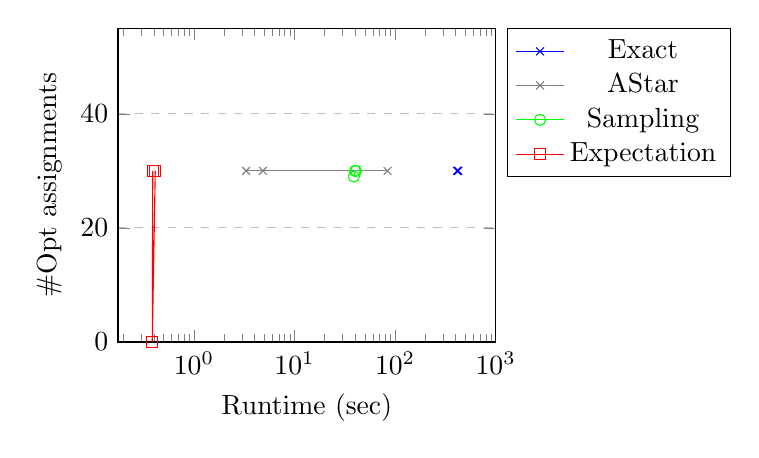
\begin{tikzpicture}
	\begin{axis}[
	scale=0.7,
	xmode=log,
	xlabel={Runtime (sec)},
	ylabel near ticks,
	ylabel={\#Opt assignments},
	xmin=0, xmax=1000,
	ymin=0, ymax=55,
	legend pos=outer north east,
	ymajorgrids=true,
	grid style=dashed,
	]
	
	\addplot[
	color=blue,
	mark=x,
	]
	coordinates { 
		(424.83 , 30) 
		(415.62 , 30) 
		(415.16 , 30) 
		
	};
	\addlegendentry{Exact}
	
	\addplot[
	color=gray,
	mark=x,
	]
	coordinates { 
		(4.854 , 30) 
		(3.306 , 30) 
		(84.209 , 30) 
		
	};
	\addlegendentry{AStar}
	
	\addplot[
	color=green,
	mark=o,
	]
	coordinates { 
		(40.93 , 30) 
		(40.016 , 30) 
		(38.929 , 29) 
		
	};
	\addlegendentry{Sampling}
	
	\addplot[
	color=red,
	mark=square,
	]
	coordinates {
		(0.413 , 30)
		(0.386 , 0) 
		(0.390 , 30) 
		
	};
	\addlegendentry{Expectation}
	
	\end{axis}
	\end{tikzpicture}
\end{figure}


\begin{figure}
	\scriptsize	
	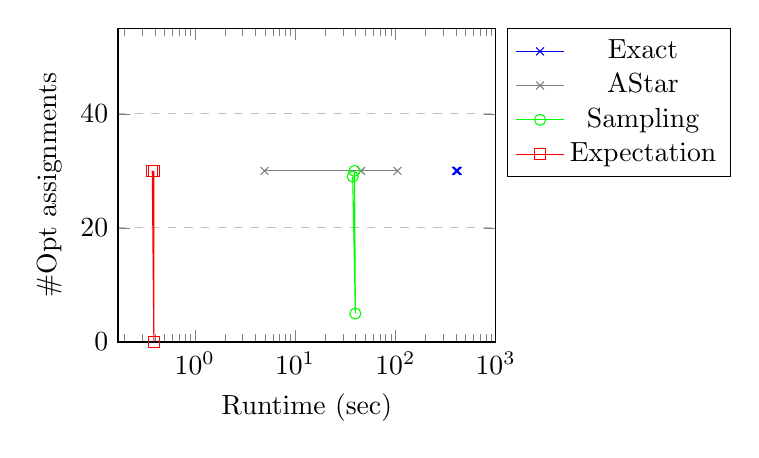
\begin{tikzpicture}
	\begin{axis}[
	scale=0.7,
	xmode=log,
	xlabel={Runtime (sec)},
	ylabel near ticks,
	ylabel={\#Opt assignments},
	xmin=0, xmax=1000,
	ymin=0, ymax=55,
	legend pos=outer north east,
	ymajorgrids=true,
	grid style=dashed,
	]
	
	\addplot[
	color=blue,
	mark=x,
	]
	coordinates { 
		(410.25 , 30) 
		(417.56 , 30) 
		(401.97 , 30) 
		
	};
	\addlegendentry{Exact}
	
	\addplot[
	color=gray,
	mark=x,
	]
	coordinates { 
		(4.956 , 30) 
		(45.518 , 30) 
		(104.75 , 30) 
		
	};
	\addlegendentry{AStar}
	
	\addplot[
	color=green,
	mark=o,
	]
	coordinates { 
		(39.11 , 30) 
		(39.89 , 5) 
		(37.54 , 29) 
		
	};
	\addlegendentry{Sampling}
	
	\addplot[
	color=red,
	mark=square,
	]
	coordinates {
		(0.390 , 30)
		(0.391 , 0) 
		(0.377 , 30) 
		
	};
	\addlegendentry{Expectation}
	
	\end{axis}
	\end{tikzpicture}
\end{figure}

\begin{figure}
	\scriptsize	
	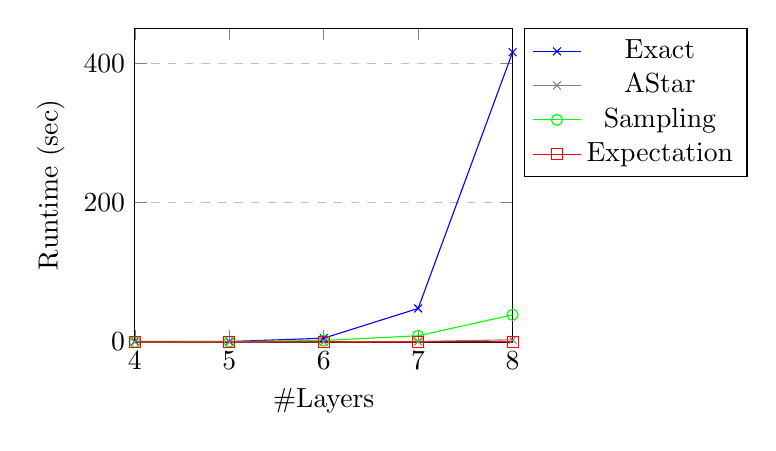
\begin{tikzpicture}
	\begin{axis}[
	scale=0.7,
	xlabel={\#Layers},
	ylabel near ticks,
	ylabel={Runtime (sec)},
	xmin=4, xmax=8,
	ymin=0, ymax=450,
	legend pos=outer north east,
	ymajorgrids=true,
	grid style=dashed,
	]
	
	\addplot[
	color=blue,
	mark=x,
	]
	coordinates { 
		(4 , 0.7) 
		(5 , 0.7) 
		(6 , 5.5)
		(7 , 48.2) 
		(8 , 415.6) 
		
	};
	\addlegendentry{Exact}
	
	\addplot[
	color=gray,
	mark=x,
	]
	coordinates { 
		(4 , 0.02) 
		(5 , 0.06) 
		(6 , 0.2)
		(7 , 0.75) 
		(8 , 3.24) 
		
	};
	\addlegendentry{AStar}
	
	\addplot[
	color=green,
	mark=o,
	]
	coordinates { 
		(4 , 0.13) 
		(5 , 0.54) 
		(6 , 2.2)
		(7 , 9) 
		(8 , 39) 
		
	};
	\addlegendentry{Sampling}
	
	\addplot[
	color=red,
	mark=square,
	]
	coordinates {
		(4 , 0.001) 
		(5 , 0.005) 
		(6 , 0.02)
		(7 , 0.09) 
		(8 , 0.4) 
		
	};
	\addlegendentry{Expectation}
	
	\end{axis}
	\end{tikzpicture}
\end{figure}

\begin{figure}
	\scriptsize	
	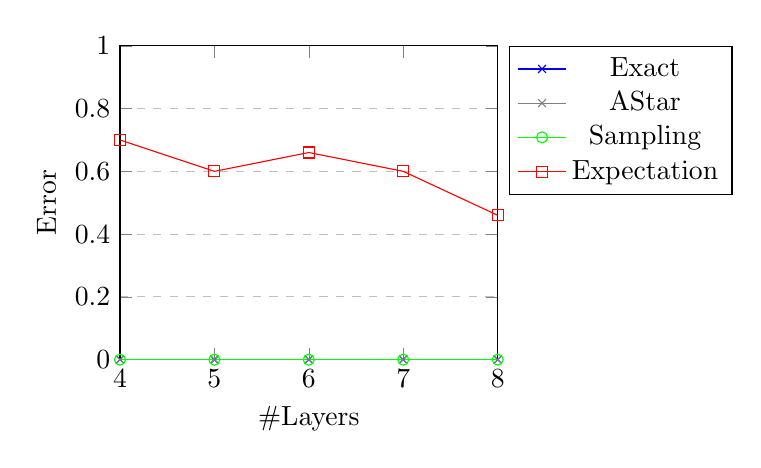
\begin{tikzpicture}
	\begin{axis}[
	scale=0.7,
	xlabel={\#Layers},
	ylabel near ticks,
	ylabel={Error},
	xmin=4, xmax=8,
	ymin=0, ymax=1,
	legend pos=outer north east,
	ymajorgrids=true,
	grid style=dashed,
	]
	
	\addplot[
	color=blue,
	mark=x,
	]
	coordinates { 
		(4 , 0) 
		(5 , 0) 
		(6 , 0)
		(7 , 0) 
		(8 , 0)
		
	};
	\addlegendentry{Exact}
	
	\addplot[
	color=gray,
	mark=x,
	]
	coordinates { 
		(4 , 0) 
		(5 , 0) 
		(6 , 0)
		(7 , 0) 
		(8 , 0)
		
	};
	\addlegendentry{AStar}
	
	\addplot[
	color=green,
	mark=o,
	]
	coordinates { 
		(4 , 0) 
		(5 , 0) 
		(6 , 0)
		(7 , 0) 
		(8 , 0)
		
	};
	\addlegendentry{Sampling}
	
	\addplot[
	color=red,
	mark=square,
	]
	coordinates {
		(4 , 0.7) 
		(5 , 0.6) 
		(6 , 0.66)
		(7 , 0.6) 
		(8 , 0.46)
		
	};
	\addlegendentry{Expectation}
	
	\end{axis}
	\end{tikzpicture}
\end{figure}

\begin{figure}
	\scriptsize	
	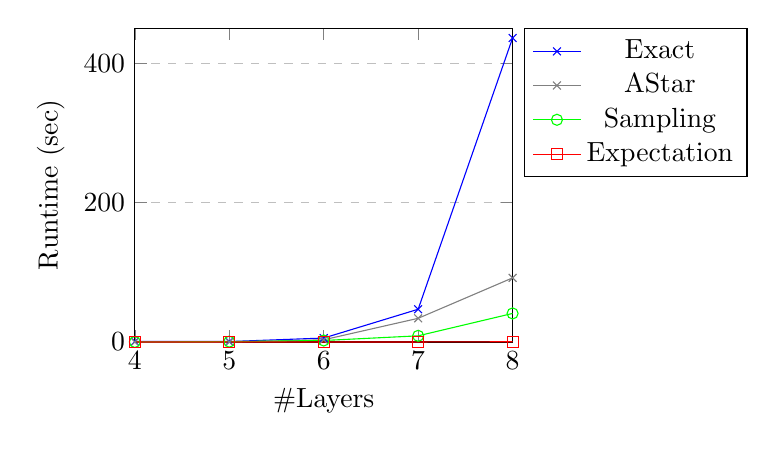
\begin{tikzpicture}
	\begin{axis}[
	scale=0.7,
	xlabel={\#Layers},
	ylabel near ticks,
	ylabel={Runtime (sec)},
	xmin=4, xmax=8,
	ymin=0, ymax=450,
	legend pos=outer north east,
	ymajorgrids=true,
	grid style=dashed,
	]
	
	\addplot[
	color=blue,
	mark=x,
	]
	coordinates { 
		(4 , 0.8) 
		(5 , 0.7) 
		(6 , 5.7)
		(7 , 47) 
		(8 , 436) 
		
	};
	\addlegendentry{Exact}
	
	\addplot[
	color=gray,
	mark=x,
	]
	coordinates { 
		(4 , 0.07) 
		(5 , 0.05) 
		(6 , 3.2)
		(7 , 34) 
		(8 , 92) 
		
	};
	\addlegendentry{AStar}
	
	\addplot[
	color=green,
	mark=o,
	]
	coordinates { 
		(4 , 0.13) 
		(5 , 0.55) 
		(6 , 2.2)
		(7 , 8.9) 
		(8 , 41) 
		
	};
	\addlegendentry{Sampling}
	
	\addplot[
	color=red,
	mark=square,
	]
	coordinates {
		(4 , 0.001) 
		(5 , 0.005) 
		(6 , 0.02)
		(7 , 0.09) 
		(8 , 0.4) 
		
	};
	\addlegendentry{Expectation}
	
	\end{axis}
	\end{tikzpicture}
\end{figure}

\begin{figure}
	\scriptsize	
	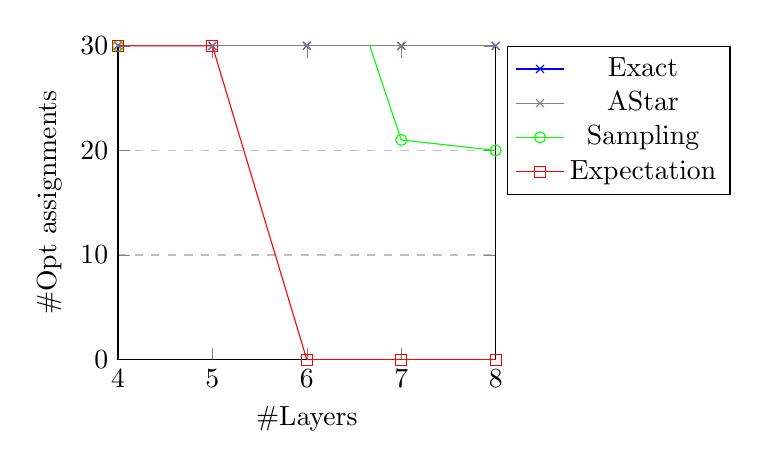
\begin{tikzpicture}
	\begin{axis}[
	scale=0.7,
	xlabel={\#Layers},
	ylabel near ticks,
	ylabel={\#Opt assignments},
	xmin=4, xmax=8,
	ymin=0, ymax=30,
	legend pos=outer north east,
	ymajorgrids=true,
	grid style=dashed,
	]
	
	\addplot[
	color=blue,
	mark=x,
	]
	coordinates { 
		(4 , 30) 
		(5 , 30) 
		(6 , 30)
		(7 , 30) 
		(8 , 30)
		
	};
	\addlegendentry{Exact}
	
	\addplot[
	color=gray,
	mark=x,
	]
	coordinates { 
		(4 , 30) 
		(5 , 30) 
		(6 , 30)
		(7 , 30) 
		(8 , 30)
		
	};
	\addlegendentry{AStar}
	
	\addplot[
	color=green,
	mark=o,
	]
	coordinates { 
		(4 , 30) 
		(5 , 48) 
		(6 , 48)
		(7 , 21) 
		(8 , 20)
		
	};
	\addlegendentry{Sampling}
	
	\addplot[
	color=red,
	mark=square,
	]
	coordinates {
		(4 , 30) 
		(5 , 30) 
		(6 , 0)
		(7 , 0) 
		(8 , 0)
		
	};
	\addlegendentry{Expectation}
	
	\end{axis}
	\end{tikzpicture}
\end{figure}


\begin{figure}
	\scriptsize	
	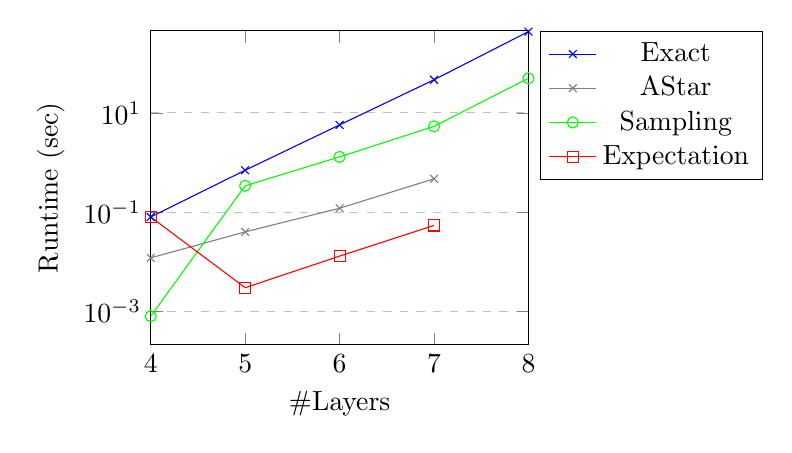
\begin{tikzpicture}
	\begin{axis}[
	scale=0.7,
	ymode = log,
	xlabel={\#Layers},
	ylabel near ticks,
	ylabel={Runtime (sec)},
	xmin=4, xmax=8,
	ymin=0, ymax=450,
	legend pos=outer north east,
	ymajorgrids=true,
	grid style=dashed,
	]
	
	\addplot[
	color=blue,
	mark=x,
	]
	coordinates { 
		(4 , 0.08) 
		(5 , 0.7) 
		(6 , 5.74)
		(7 , 46.6) 
		(8 , 436) 
		
	};
	\addlegendentry{Exact}
	
	\addplot[
	color=gray,
	mark=x,
	]
	coordinates { 
		(4 , 0.012) 
		(5 , 0.04) 
		(6 , 0.12)
		(7 , 0.47) 

	};
	\addlegendentry{AStar}
	
	
		\addplot[
	color=green,
	mark=o,
	]
	coordinates { 
		(4 , 0.0008) 
		(5 , 0.34) 
		(6 , 1.3)
		(7 , 5.36) 
		(8 , 50) 
		
	};
	\addlegendentry{Sampling}
	
	\addplot[
	color=red,
	mark=square,
	]
	coordinates {
		(4 , 0.08) 
		(5 , 0.003) 
		(6 , 0.013)
		(7 , 0.054) 

	};
	\addlegendentry{Expectation}
	
	\end{axis}
	\end{tikzpicture}
	\caption{Run time comparison of all heuristic algorithms for deadline of size $0.5\cdot$ MaxDeadline and ``Failure" distribution}\label{05failrt}
\end{figure}
\begin{figure}
	\scriptsize	
	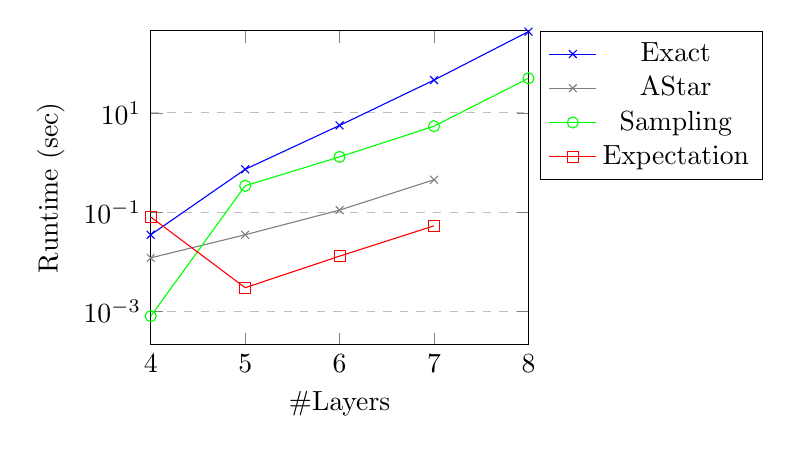
\begin{tikzpicture}
	\begin{axis}[
	scale=0.7,
	ymode = log,
	xlabel={\#Layers},
	ylabel near ticks,
	ylabel={Runtime (sec)},
	xmin=4, xmax=8,
	ymin=0, ymax=450,
	legend pos=outer north east,
	ymajorgrids=true,
	grid style=dashed,
	]
	
	\addplot[
	color=blue,
	mark=x,
	]
	coordinates { 
		(4 , 0.035) 
		(5 , 0.73) 
		(6 , 5.6)
		(7 , 46) 
		(8 , 436) 
		
	};
	\addlegendentry{Exact}
	
	\addplot[
	color=gray,
	mark=x,
	]
	coordinates { 
		(4 , 0.012) 
		(5 , 0.035) 
		(6 , 0.11)
		(7 , 0.45) 

	};
	\addlegendentry{AStar}
	
	
		\addplot[
	color=green,
	mark=o,
	]
	coordinates { 
		(4 , 0.0008) 
		(5 , 0.34) 
		(6 , 1.3)
		(7 , 5.4) 
		(8 , 50) 
		
	};
	\addlegendentry{Sampling}
	
	\addplot[
	color=red,
	mark=square,
	]
	coordinates {
		(4 , 0.08) 
		(5 , 0.003) 
		(6 , 0.013)
		(7 , 0.053) 

	};
	\addlegendentry{Expectation}
	
	\end{axis}
	\end{tikzpicture}
	\caption{Run time comparison of all heuristic algorithms for deadline of size $0.75\cdot$ MaxDeadline and ``Failure" distribution}\label{075failrt}
\end{figure}
\begin{figure}
	\scriptsize	
	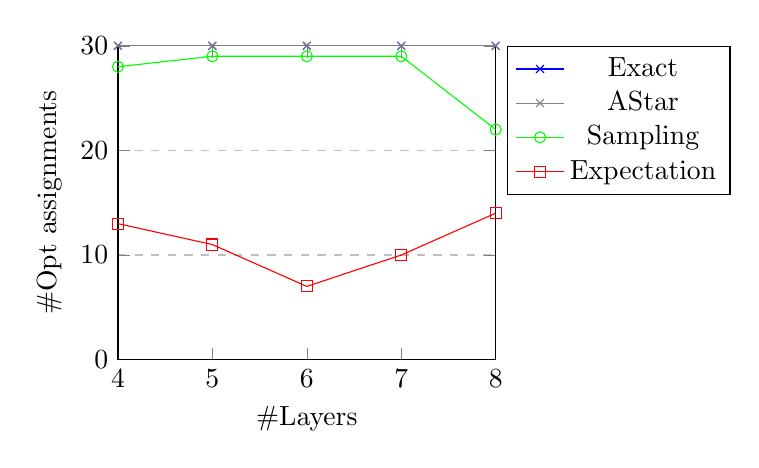
\begin{tikzpicture}
	\begin{axis}[
	scale=0.7,
	xlabel={\#Layers},
	ylabel near ticks,
	ylabel={\#Opt assignments},
	xmin=4, xmax=8,
	ymin=0, ymax=30,
	legend pos=outer north east,
	ymajorgrids=true,
	grid style=dashed,
	]
	
	\addplot[
	color=blue,
	mark=x,
	]
	coordinates { 
		(4 , 30) 
		(5 , 30) 
		(6 , 30)
		(7 , 30) 
		(8 , 30)
		
	};
	\addlegendentry{Exact}
	
	\addplot[
	color=gray,
	mark=x,
	]
	coordinates { 
		(4 , 30) 
		(5 , 30) 
		(6 , 30)
		(7 , 30) 
		(8 , 30)
		
	};
	\addlegendentry{AStar}
	
	\addplot[
	color=green,
	mark=o,
	]
	coordinates { 
		(4 , 28) 
		(5 , 29) 
		(6 , 29)
		(7 , 29) 
		(8 , 22)

	};
	\addlegendentry{Sampling}
	
	\addplot[
	color=red,
	mark=square,
	]
	coordinates {
		(4 , 13) 
		(5 , 11) 
		(6 , 7)
		(7 , 10) 
		(8, 14)

	};
	\addlegendentry{Expectation}
	
	\end{axis}
	\end{tikzpicture}
	\caption{Number of optimal assingments comparison of all heuristic algorithms for deadline of size $0.25\cdot$ MaxDeadline and random distribution}
\end{figure}




\begin{figure}
	\scriptsize	
	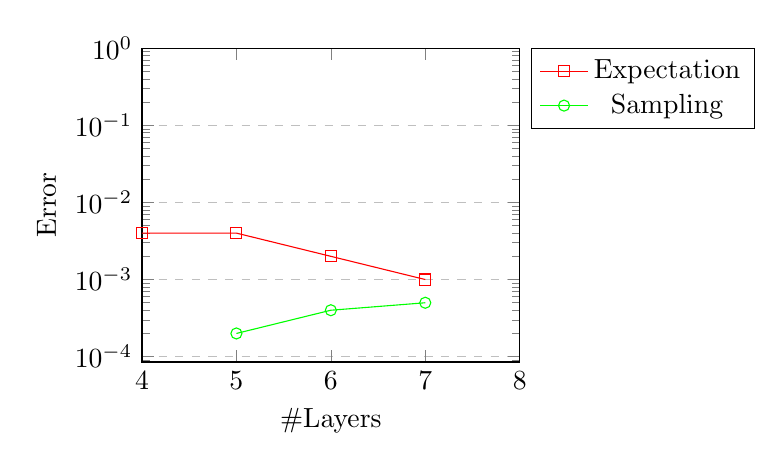
\begin{tikzpicture}
	\begin{axis}[
	scale=0.7,
	ymode=log,
	xlabel={\#Layers},
	ylabel near ticks,
	ylabel={Error},
	xmin=4, xmax=8,
	ymin=0, ymax=1,
	legend pos=outer north east,
	ymajorgrids=true,
	grid style=dashed,
	]
	
	\addplot[
	color=red,
	mark=square,
	]
	coordinates {
		(4 , 0.004) 
		(5 , 0.004) 
		(6 , 0.002)
		(7 , 0.001) 

	};
	\addlegendentry{Expectation}
	
	\addplot[
	color=green,
	mark=o,
	]
	coordinates { 
		(4 , 0) 
		(5 , 0.0002) 
		(6 , 0.0004)
		(7 , 0.0005) 

	};
	\addlegendentry{Sampling}
	
	\end{axis}
	\end{tikzpicture}
	\caption{Error comparison of all heuristic algorithms for deadline of size $0.5\cdot$ MaxDeadline and random distribution}
\end{figure}



\begin{figure}
	\scriptsize	
	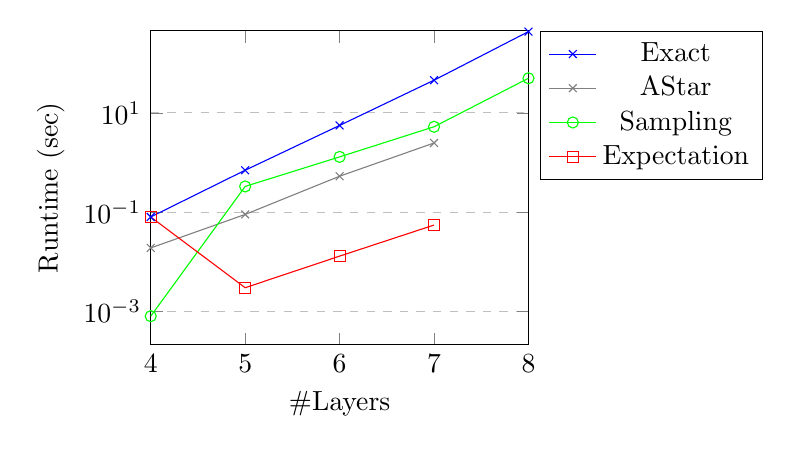
\begin{tikzpicture}
	\begin{axis}[
	scale=0.7,
	ymode=log,
	xlabel={\#Layers},
	ylabel near ticks,
	ylabel={Runtime (sec)},
	xmin=4, xmax=8,
	ymin=0, ymax=450,
	legend pos=outer north east,
	ymajorgrids=true,
	grid style=dashed,
	]
	
	\addplot[
	color=blue,
	mark=x,
	]
	coordinates { 
		(4 , 0.08) 
		(5 , 0.7) 
		(6 , 5.6)
		(7 , 45.7) 
		(8 , 436) 
		
	};
	\addlegendentry{Exact}
	
	\addplot[
	color=gray,
	mark=x,
	]
	coordinates { 
		(4 , 0.019) 
		(5 , 0.09) 
		(6 , 0.53)
		(7 , 2.48) 

	};
	\addlegendentry{AStar}
	
	
		\addplot[
	color=green,
	mark=o,
	]
	coordinates { 
		(4 , 0.0008) 
		(5 , 0.33) 
		(6 , 1.3)
		(7 , 5.26) 
		(8 , 50) 
		
	};
	\addlegendentry{Sampling}
	
	\addplot[
	color=red,
	mark=square,
	]
	coordinates {
		(4 , 0.08) 
		(5 , 0.003) 
		(6 , 0.013)
		(7 , 0.055) 

	};
	\addlegendentry{Expectation}

	
	\end{axis}
	\end{tikzpicture}
	\caption{Run time comparison of all heuristic algorithms for deadline of size $0.5\cdot$ MaxDeadline and random distribution}
\end{figure}



























\begin{figure}
	\scriptsize	
	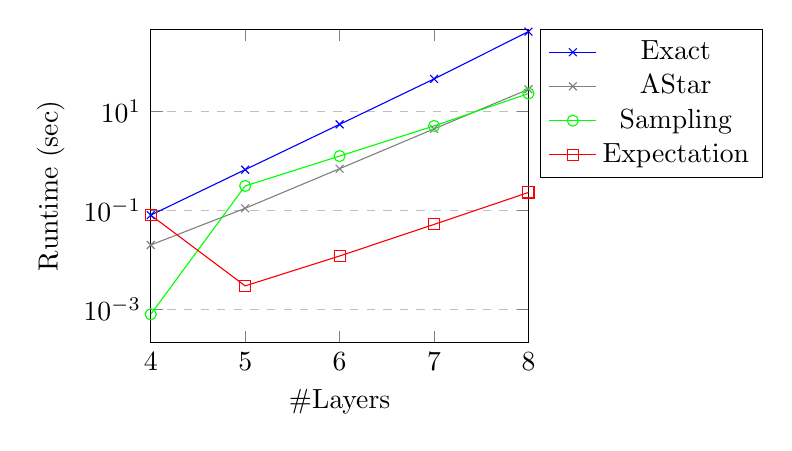
\begin{tikzpicture}
	\begin{axis}[
	scale=0.7,
	ymode = log,
	xlabel={\#Layers},
	ylabel near ticks,
	ylabel={Runtime (sec)},
	xmin=4, xmax=8,
	ymin=0, ymax=450,
	legend pos=outer north east,
	ymajorgrids=true,
	grid style=dashed,
	]
	
	\addplot[
	color=blue,
	mark=x,
	]
	coordinates { 
		(4 , 0.08) 
		(5 , 0.66) 
		(6 , 5.4)
		(7 , 44.48) 
		(8 , 400.3) 
		
	};
	\addlegendentry{Exact}
	
	\addplot[
	color=gray,
	mark=x,
	]
	coordinates { 
		(4 , 0.02) 
		(5 , 0.11) 
		(6 , 0.69)
		(7 , 4.38) 
		(8 , 27.53)

	};
	\addlegendentry{AStar}
	
	
		\addplot[
	color=green,
	mark=o,
	]
	coordinates { 
		(4 , 0.0008) 
		(5 , 0.31) 
		(6 , 1.24)
		(7 , 5.02) 
		(8 , 22.6) 
		
	};
	\addlegendentry{Sampling}
	
	\addplot[
	color=red,
	mark=square,
	]
	coordinates {
		(4 , 0.08) 
		(5 , 0.003) 
		(6 , 0.012)
		(7 , 0.052) 
		(8 , 0.229)

	};
	\addlegendentry{Expectation}
	
	\end{axis}
	\end{tikzpicture}
	\caption{Run time comparison of all heuristic algorithms for deadline of size $0.25\cdot$ MaxDeadline and ''Structural" distribution}
\end{figure}


\begin{figure}
	\scriptsize	
	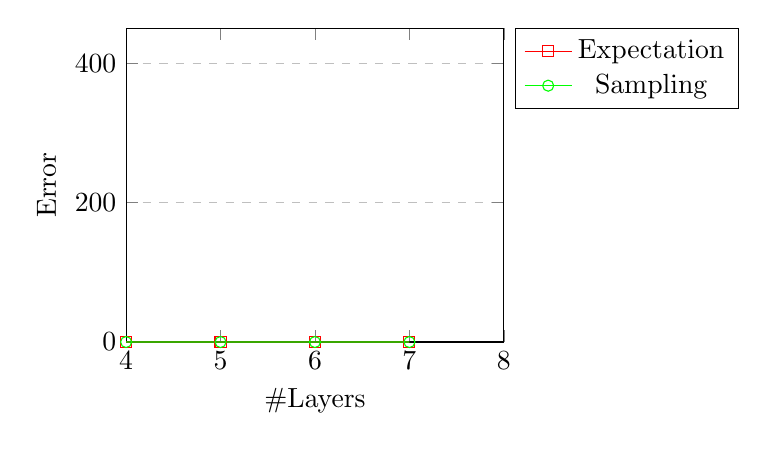
\begin{tikzpicture}
	\begin{axis}[
	scale=0.7,
	xlabel={\#Layers},
	ylabel near ticks,
	ylabel={Error},
	xmin=4, xmax=8,
	ymin=0, ymax=450,
	legend pos=outer north east,
	ymajorgrids=true,
	grid style=dashed,
	]
	
	\addplot[
	color=red,
	mark=square,
	]
	coordinates {
		(4 , 0.001) 
		(5 , 0.001) 
		(6 , 0.0005)
		(7 , 0.0003) 

	};
	\addlegendentry{Expectation}
	
	
	\addplot[
	color=green,
	mark=o,
	]
	coordinates { 
		(4 , 0) 
		(5 , 0.0002) 
		(6 , 0.0004)
		(7 , 0.003) 

	};
	\addlegendentry{Sampling}
	
	\end{axis}
	\end{tikzpicture}
	\caption{Error comparison of all heuristic algorithms for deadline of size $0.5\cdot$ MaxDeadline and ''Structural" distribution}
\end{figure}



\begin{figure}
	\scriptsize	
	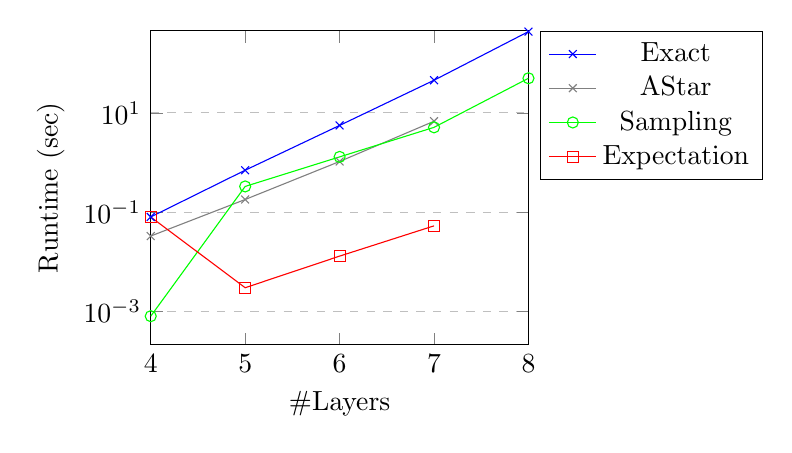
\begin{tikzpicture}
	\begin{axis}[
	scale=0.7,
	ymode = log,
	xlabel={\#Layers},
	ylabel near ticks,
	ylabel={Runtime (sec)},
	xmin=4, xmax=8,
	ymin=0, ymax=450,
	legend pos=outer north east,
	ymajorgrids=true,
	grid style=dashed,
	]
	
	\addplot[
	color=blue,
	mark=x,
	]
	coordinates { 
		(4 , 0.08) 
		(5 , 0.7) 
		(6 , 5.6)
		(7 , 45.6) 
		(8 , 436) 
		
	};
	\addlegendentry{Exact}
	
	\addplot[
	color=gray,
	mark=x,
	]
	coordinates { 
		(4 , 0.033) 
		(5 , 0.18) 
		(6 , 1.05)
		(7 , 6.8) 

	};
	\addlegendentry{AStar}
	
	
		\addplot[
	color=green,
	mark=o,
	]
	coordinates { 
		(4 , 0.0008) 
		(5 , 0.33) 
		(6 , 1.3)
		(7 , 5.12) 
		(8 , 50) 
		
	};
	\addlegendentry{Sampling}
	
	\addplot[
	color=red,
	mark=square,
	]
	coordinates {
		(4 , 0.08) 
		(5 , 0.003) 
		(6 , 0.013)
		(7 , 0.053) 

	};
	\addlegendentry{Expectation}
	
	\end{axis}
	\end{tikzpicture}
	\caption{Run time comparison of all heuristic algorithms for deadline of size $0.5\cdot$ MaxDeadline and ''Structural" distribution}
\end{figure}



\begin{figure}
	\scriptsize	
	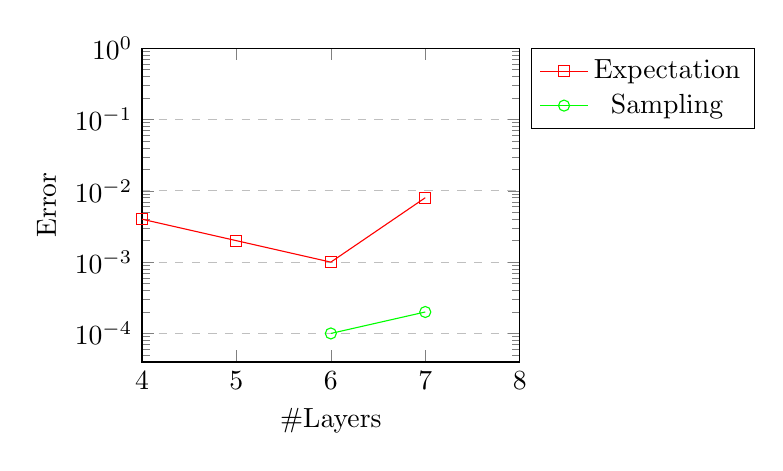
\begin{tikzpicture}
	\begin{axis}[
	scale=0.7,
	ymode = log,
	xlabel={\#Layers},
	ylabel near ticks,
	ylabel={Error},
	xmin=4, xmax=8,
	ymin=0, ymax=1,
	legend pos=outer north east,
	ymajorgrids=true,
	grid style=dashed,
	]
	
	\addplot[
	color=red,
	mark=square,
	]
	coordinates {
		(4 , 0.004) 
		(5 , 0.002) 
		(6 , 0.001)
		(7 , 0.008) 

	};
	\addlegendentry{Expectation}
	
	\addplot[
	color=green,
	mark=o,
	]
	coordinates { 
		(4 , 0) 
		(5 , 0) 
		(6 , 0.0001)
		(7 , 0.0002) 

	};
	\addlegendentry{Sampling}
	
	
	
	\end{axis}
	\end{tikzpicture}
	\caption{Error comparison of all heuristic algorithms for deadline of size $0.75\cdot$ MaxDeadline and ''Structural" distribution}
\end{figure}




\begin{figure}
	\scriptsize	
	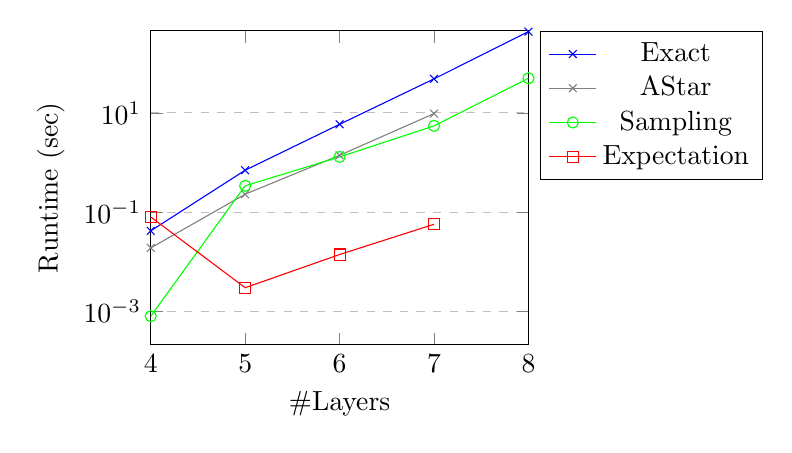
\begin{tikzpicture}
	\begin{axis}[
	scale=0.7,
	ymode = log,
	xlabel={\#Layers},
	ylabel near ticks,
	ylabel={Runtime (sec)},
	xmin=4, xmax=8,
	ymin=0, ymax=450,
	legend pos=outer north east,
	ymajorgrids=true,
	grid style=dashed,
	]
	
	\addplot[
	color=blue,
	mark=x,
	]
	coordinates { 
		(4 , 0.042) 
		(5 , 0.7) 
		(6 , 5.9)
		(7 , 48.6) 
		(8 , 436) 
		
	};
	\addlegendentry{Exact}
	
	\addplot[
	color=gray,
	mark=x,
	]
	coordinates { 
		(4 , 0.019) 
		(5 , 0.23) 
		(6 , 1.4)
		(7 , 9.7) 

	};
	\addlegendentry{AStar}
	
	
		\addplot[
	color=green,
	mark=o,
	]
	coordinates { 
		(4 , 0.0008) 
		(5 , 0.34) 
		(6 , 1.3)
		(7 , 5.48) 
		(8 , 50) 
		
	};
	\addlegendentry{Sampling}
	
	\addplot[
	color=red,
	mark=square,
	]
	coordinates {
		(4 , 0.08) 
		(5 , 0.003) 
		(6 , 0.014)
		(7 , 0.057) 

	};
	\addlegendentry{Expectation}
	
	\end{axis}
	\end{tikzpicture}
	\caption{Run time comparison of all heuristic algorithms for deadline of size $0.75\cdot$ MaxDeadline and ''Structural" distribution}
\end{figure}


\begin{figure}
	\scriptsize	
	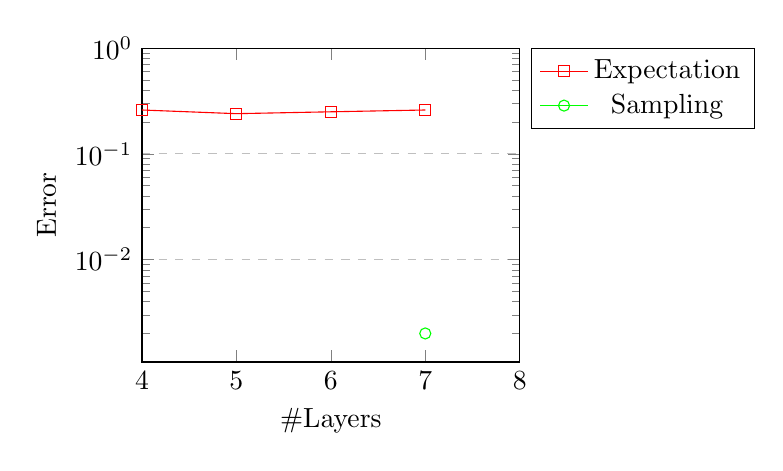
\begin{tikzpicture}
	\begin{axis}[
	scale=0.7,
	ymode=log,
	xlabel={\#Layers},
	ylabel near ticks,
	ylabel={Error},
	xmin=4, xmax=8,
	ymin=0, ymax=1,
	legend pos=outer north east,
	ymajorgrids=true,
	grid style=dashed,
	]
	
	\addplot[
	color=red,
	mark=square,
	]
	coordinates {
		(4 , 0.26) 
		(5 , 0.24) 
		(6 , 0.25)
		(7 , 0.26) 

	};
	\addlegendentry{Expectation}
	
	\addplot[
	color=green,
	mark=o,
	]
	coordinates { 
		(4 , 0) 
		(5 , 0) 
		(6 , 0)
		(7 , 0.002) 

	};
	\addlegendentry{Sampling}
	
	
	\end{axis}
	\end{tikzpicture}
	\caption{Error comparison of all heuristic algorithms for deadline of size $0.5\cdot$ MaxDeadline and ``Failure" distribution}\label{05faile}
\end{figure}


\begin{figure}
	\scriptsize	
	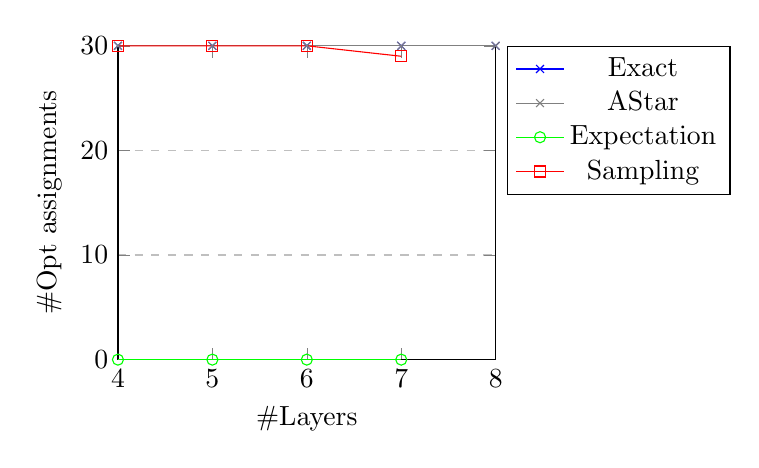
\begin{tikzpicture}
	\begin{axis}[
	scale=0.7,
	xlabel={\#Layers},
	ylabel near ticks,
	ylabel={\#Opt assignments},
	xmin=4, xmax=8,
	ymin=0, ymax=30,
	legend pos=outer north east,
	ymajorgrids=true,
	grid style=dashed,
	]
	
	\addplot[
	color=blue,
	mark=x,
	]
	coordinates { 
		(4 , 30) 
		(5 , 30) 
		(6 , 30)
		(7 , 30) 
		(8 , 30)
		
	};
	\addlegendentry{Exact}
	
	\addplot[
	color=gray,
	mark=x,
	]
	coordinates { 
		(4 , 30) 
		(5 , 30) 
		(6 , 30)
		(7 , 30) 
		(8 , 30)
		
	};
	\addlegendentry{AStar}
	
	\addplot[
	color=green,
	mark=o,
	]
	coordinates { 
		(4 , 0) 
		(5 , 0) 
		(6 , 0)
		(7 , 0) 

	};
	\addlegendentry{Expectation}
	
	\addplot[
	color=red,
	mark=square,
	]
	coordinates {
		(4 , 30) 
		(5 , 30) 
		(6 , 30)
		(7 , 29) 

	};
	\addlegendentry{Sampling}
	
	\end{axis}
	\end{tikzpicture}
	\caption{Number of optimal assingments comparison of all heuristic algorithms for deadline of size $0.5\cdot$ MaxDeadline and ``Failure" distribution}\label{05failn}
\end{figure}

\begin{figure}
	\scriptsize	
	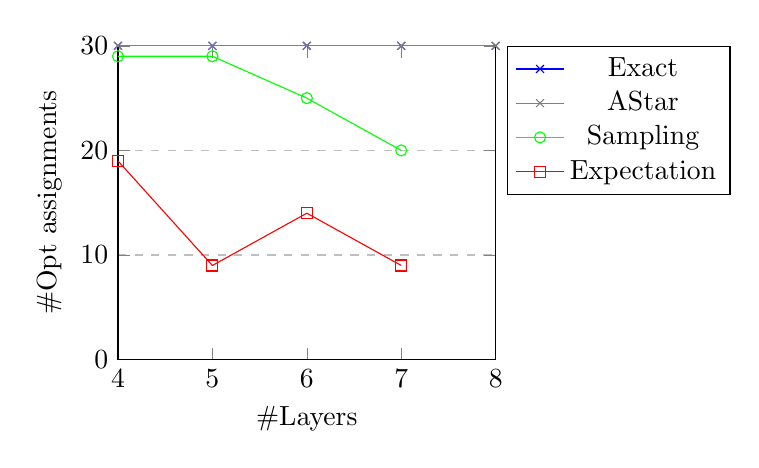
\begin{tikzpicture}
	\begin{axis}[
	scale=0.7,
	xlabel={\#Layers},
	ylabel near ticks,
	ylabel={\#Opt assignments},
	xmin=4, xmax=8,
	ymin=0, ymax=30,
	legend pos=outer north east,
	ymajorgrids=true,
	grid style=dashed,
	]
	
	\addplot[
	color=blue,
	mark=x,
	]
	coordinates { 
		(4 , 30) 
		(5 , 30) 
		(6 , 30)
		(7 , 30) 
		(8 , 30)
		
	};
	\addlegendentry{Exact}
	
	\addplot[
	color=gray,
	mark=x,
	]
	coordinates { 
		(4 , 30) 
		(5 , 30) 
		(6 , 30)
		(7 , 30) 
		(8 , 30)
		
	};
	\addlegendentry{AStar}
	
	\addplot[
	color=green,
	mark=o,
	]
	coordinates { 
		(4 , 29) 
		(5 , 29) 
		(6 , 25)
		(7 , 20) 

	};
	\addlegendentry{Sampling}
	
	\addplot[
	color=red,
	mark=square,
	]
	coordinates {
		(4 , 19) 
		(5 , 9) 
		(6 , 14)
		(7 , 9) 

	};
	\addlegendentry{Expectation}
	
	\end{axis}
	\end{tikzpicture}
	\caption{Number of optimal assingments comparison of all heuristic algorithms for deadline of size $0.75\cdot$ MaxDeadline and random distribution}
\end{figure}






\begin{figure}
	\scriptsize	
	\begin{tikzpicture}
	\begin{axis}[
	scale=0.7,
	xlabel={\#Layers},
	ylabel near ticks,
	ylabel={\#Opt assignments},
	xmin=4, xmax=8,
	ymin=0, ymax=30,
	legend pos=outer north east,
	ymajorgrids=true,
	grid style=dashed,
	]
	
	\addplot[
	color=blue,
	mark=x,
	]
	coordinates { 
		(4 , 30) 
		(5 , 30) 
		(6 , 30)
		(7 , 30) 
		(8 , 30)
		
	};
	\addlegendentry{BF}
	
	\addplot[
	color=gray,
	mark=x,
	]
	coordinates { 
		(4 , 30) 
		(5 , 30) 
		(6 , 30)
		(7 , 30) 
		(8 , 30)
		
	};
	\addlegendentry{\astar}
	
	\addplot[
	color=green,
	mark=o,
	]
	coordinates { 
		(4 , 30) 
		(5 , 29) 
		(6 , 28)
		(7 , 29) 

	};
	\addlegendentry{\sampling}
	
	\addplot[
	color=red,
	mark=square,
	]
	coordinates {
		(4 , 25) 
		(5 , 18) 
		(6 , 21)
		(7 , 25) 

	};
	\addlegendentry{\expectation}
	
	\end{axis}
	\end{tikzpicture}
	\caption{Number of optimal assingments comparison of all heuristic algorithms for deadline of size $0.5\cdot$ MaxDeadline and random distribution}\label{05rand}
\end{figure}



\begin{figure}
	\scriptsize	
	\begin{tikzpicture}
	\begin{axis}[
	scale=0.7,
	xlabel={\#Layers},
	ylabel near ticks,
	ylabel={\#Opt assignments},
	xmin=4, xmax=8,
	ymin=0, ymax=30,
	legend pos=outer north east,
	ymajorgrids=true,
	grid style=dashed,
	]
	
	\addplot[
	color=blue,
	mark=x,
	]
	coordinates { 
		(4 , 30) 
		(5 , 30) 
		(6 , 30)
		(7 , 30) 
		(8 , 30)
		
	};
	\addlegendentry{BF}
	
	\addplot[
	color=gray,
	mark=x,
	]
	coordinates { 
		(4 , 30) 
		(5 , 30) 
		(6 , 30)
		(7 , 30) 
		(8 , 30)
		
	};
	\addlegendentry{\astar}
	
	\addplot[
	color=green,
	mark=o,
	]
	coordinates { 
		(4 , 0) 
		(5 , 0) 
		(6 , 0)
		(7 , 0) 
		(8 , 0)

	};
	\addlegendentry{\expectation}
	
	\addplot[
	color=red,
	mark=square,
	]
	coordinates {
		(4 , 30) 
		(5 , 29) 
		(6 , 30)
		(7 , 29) 
		(8 , 26)

	};
	\addlegendentry{\sampling}
	
	\end{axis}
	\end{tikzpicture}
	\caption{Number of optimal assingments comparison of all heuristic algorithms for deadline of size $0.25\cdot$ MaxDeadline and ``Failure" distribution}\label{025failn}
\end{figure}




\begin{figure}
	\scriptsize	
	\begin{tikzpicture}
	\begin{axis}[
	scale=0.7,
	ymode=log,
	xlabel={\#Layers},
	ylabel near ticks,
	ylabel={Error},
	xmin=4, xmax=8,
	ymin=0, ymax=1,
	legend pos=outer north east,
	ymajorgrids=true,
	grid style=dashed,
	]
	
	\addplot[
	color=red,
	mark=square,
	]
	coordinates {
		(4 , 0.022) 
		(5 , 0.02) 
		(6 , 0.014)
		(7 , 0.008) 
		(8 ,0.0068)

	};
	\addlegendentry{\expectation}
	
	\addplot[
	color=green,
	mark=o,
	]
	coordinates { 
		(4 , 0) 
		(5 , 0.00002) 
		(6 , 0)
		(7 , 0.00003) 
		(8 , 0.00006)

	};
	\addlegendentry{\sampling}
	
	
	
	\end{axis}
	\end{tikzpicture}
	\caption{Error comparison of all heuristic algorithms for deadline of size $0.25\cdot$ MaxDeadline and ``Failure" distribution}\label{025faile}
\end{figure}



\begin{figure}
	\scriptsize	
	\begin{tikzpicture}
	\begin{axis}[
	scale=0.7,
	xlabel={\#Layers},
	ylabel near ticks,
	ylabel={\#Opt assignments},
	xmin=4, xmax=8,
	ymin=0, ymax=30,
	legend pos=outer north east,
	ymajorgrids=true,
	grid style=dashed,
	]
	
	\addplot[
	color=blue,
	mark=x,
	]
	coordinates { 
		(4 , 30) 
		(5 , 30) 
		(6 , 30)
		(7 , 30) 
		(8 , 30)
		
	};
	\addlegendentry{BF}
	
	\addplot[
	color=gray,
	mark=x,
	]
	coordinates { 
		(4 , 30) 
		(5 , 30) 
		(6 , 30)
		(7 , 30) 
		(8 , 30)
		
	};
	\addlegendentry{\astar}
	
	\addplot[
	color=red,
	mark=square,
	]
	coordinates { 
		(4 , 15) 
		(5 , 9) 
		(6 , 6)
		(7 , 7) 
		(8 , 4)

	};
	\addlegendentry{\expectation}
	
	\addplot[
	color=green,
	mark=o,
	]
	coordinates {
		(4 , 30) 
		(5 , 30) 
		(6 , 24)
		(7 , 22) 
		(8 , 19)

	};
	\addlegendentry{\sampling}
	
	\end{axis}
	\end{tikzpicture}
	\caption{Number of optimal assingments comparison of all heuristic algorithms for deadline of size $0.25\cdot$ MaxDeadline and ``Structural" distribution}
\end{figure}\label{025regrt}

